\documentclass{article}
\usepackage{graphicx}
\usepackage[utf8]{inputenc}
\usepackage{fullpage}
\usepackage{float}
\restylefloat{figure}
\usepackage[frenchb]{babel}
\usepackage{xcolor,listings}
\usepackage{color}
\definecolor{maroon}{rgb}{0.5,0,0}
\definecolor{darkgreen}{rgb}{0,0.5,0}
\usepackage[acronym]{glossaries}
\makeglossaries

\usepackage{listings}

\lstdefinelanguage{XML}
{
  basicstyle=\normalfont\ttfamily,
  numbers=left,
  numberstyle=\scriptsize,
  stepnumber=1,
  numbersep=8pt,
  showstringspaces=false,
  breaklines=true,
  frame=lines,
  backgroundcolor=\color{background},
  morestring=[s]{"}{"},
  morecomment=[s]{?}{?},
  morecomment=[s]{!--}{--},
  commentstyle=\color{darkgreen},
  moredelim=[s][\color{black}]{>}{<},
  moredelim=[s][\color{red}]{\ }{=},
  stringstyle=\color{blue},
  captionpos=b,
  identifierstyle=\color{maroon}
}
\colorlet{punct}{red!60!black}
\definecolor{background}{HTML}{EEEEEE}
\definecolor{delim}{RGB}{20,105,176}
\colorlet{numb}{magenta!60!black}

\lstdefinelanguage{json}{
    basicstyle=\normalfont\ttfamily,
    captionpos=b,
    numbers=left,
    numberstyle=\scriptsize,
    stepnumber=1,
    numbersep=8pt,
    showstringspaces=false,
    breaklines=true,
    frame=lines,
    stringstyle=\color{blue},
    morestring=[s]{"}{"},
    backgroundcolor=\color{background},
    literate=
     *{0}{{{\color{blue}0}}}{1}
      {1}{{{\color{blue}1}}}{1}
      {2}{{{\color{blue}2}}}{1}
      {3}{{{\color{blue}3}}}{1}
      {4}{{{\color{blue}4}}}{1}
      {5}{{{\color{blue}5}}}{1}
      {6}{{{\color{blue}6}}}{1}
      {7}{{{\color{blue}7}}}{1}
      {8}{{{\color{blue}8}}}{1}
      {9}{{{\color{blue}9}}}{1}
      {:}{{{\color{punct}{:}}}}{1}
      {,}{{{\color{punct}{,}}}}{1}
      {\{}{{{\color{delim}{\{}}}}{1}
      {\}}{{{\color{delim}{\}}}}}{1}
      {[}{{{\color{delim}{[}}}}{1}
      {]}{{{\color{delim}{]}}}}{1},
}

\definecolor{dkgreen}{rgb}{0,0.6,0}
\definecolor{dred}{rgb}{0.545,0,0}
\definecolor{dblue}{rgb}{0,0,0.545}
\definecolor{lgrey}{rgb}{0.9,0.9,0.9}
\definecolor{gray}{rgb}{0.4,0.4,0.4}
\definecolor{darkblue}{rgb}{0.0,0.0,0.6}
\lstdefinelanguage{cpp}{
      backgroundcolor=\color{lgrey},  
      basicstyle=\footnotesize \ttfamily \color{black} \bfseries,   
      breakatwhitespace=false,       
      breaklines=true,               
      captionpos=b,                   
      commentstyle=\color{dkgreen},   
      deletekeywords={...},          
      escapeinside={\%*}{*)},                  
      frame=single,                  
      language=C++,                
      keywordstyle=\color{purple},  
      morekeywords={BRIEFDescriptorConfig,string,TiXmlNode,DetectorDescriptorConfigContainer,istringstream,cerr,exit}, 
      identifierstyle=\color{black},
      stringstyle=\color{blue},      
      numbers=right,                 
      numbersep=5pt,                  
      numberstyle=\tiny\color{black}, 
      rulecolor=\color{black},        
      showspaces=false,               
      showstringspaces=false,        
      showtabs=false,                
      stepnumber=1,                   
      tabsize=5,                     
    }


\begin{document}

	\begin{titlepage}
		\begin{center}
		
			
\includegraphics[scale=0.4]{cuda_logo.jpg}
			\hspace*{3in}
			
\includegraphics[scale=0.08]{angers.jpg}
			\\[4cm]
			\begin{Huge}
				\rule{\linewidth}{0.5mm} \\[0.4cm]
				CUDAisation du code impératif
				\rule{\linewidth}{0.5mm} \\[0.3cm]
				
			\end{Huge}
			\begin{Large}
				POC (Proof of Concept) pour la génération de kernel à partir de code impératif
			\end{Large}		
			 
		\end{center}
		
		
  		\begin{figure}[b]
  		 \begin{minipage}{0.4\textwidth}
			\begin{flushleft} \large
				Alexis BRIARD\\
				Guillaume GRANDJEAN\\
				Jason JAMET
    		\end{flushleft}
    		\end{minipage}
    		\begin{minipage}{0.6\textwidth}
			\begin{flushright} \large
				\emph{Tuteur pédagogique:} Jean Michel RICHER\\				
        		Université d'Angers\\
        		\today
    		\end{flushright}
    	\end{minipage}
		\end{figure}

    	
	\end{titlepage}

\newpage
\thispagestyle{empty}
\mbox{}
\setcounter{page}{0}
\glsresetall
\newpage
\tableofcontents
\newpage

	\section{Présentation}

	\subsection{Objectifs}

	\paragraph{}
	Le but du projet était de réaliser une étude de faisabilité, ou POC (Proof of Concept) afin de montrer comment transformer du code impératif vers CUDA, une technologie de nVidia pour faire du calcul parallèle.
	
	\begin{lstlisting}[
    language=cpp,
]
#pragma cuda thread_loop(i) params(x,y,z,size) 
void sum(float *x, float *y, float *z, int size) { 
	for (int i=0; i<size; ++i) {
		z[i] = x[i] + y[i];
	}
}

_____________________________________


__global__ void kernel(float *x, float *y, float *z, int size) { 
	int gtid = ...
	if (gtid < size) {
		z[i] = x[i] + y[i];
	}
}
	
	\end{lstlisting}	
	
	\subsection{Technologies et outils utilisés}
	
	Pour ce projet, comme nous le verrons plus tard, nous sommes partis d'un projet déjà existant implémenté en \verb|C++|, nous avons donc utilisé ce langage pour la structure de l'arbre réalisé.
	Pour le parseur, nous avons utilisé les technologies \verb|bison| et \verb|flex|, que nous avions déjà utilisé lors d'un précédent projet.
	Enfin, étant 3 personnes à travailler sur les mêmes fichiers, nous avons utilisé le système de gestion de version \verb|Git|, qui nous permet de garder les fichiers modifiés et de faciliter le travail.
	
	\newpage	
	
	\section{Analyse du problème}
	
	\subsection{Analyse générale}
	
	Nous avons commencé par identifier les différents cas que nous pourrions rencontrer lors de la transformation d'une fonction lambda vers CUDA, ainsi nous avons pu établir une liste des paramètres qui influent sur la transformation.
	\\Prenons une fonction simple à traduire en kernel
		\begin{lstlisting}[
    language=cpp,
]
#pragma cuda thread_loop(i) 
void sum(float *x, float *y, float *z, int size) { 
	int i;
	for (i=0; i<size; ++i) {
			z[i] = x[i] + y[i];
	}
}

_____________________________________


__global__ void kernel(float *x, float *y, float *z, int size) { 
	int i = ((((blockIdx.x * gridDim.y + blockIdx.y) * gridDim.z + blockIdx.z) * blockDim.x + threadIdx.x) * blockDim.y + threadIdx.y) * blockDim.z + threadIdx.z;
	if (i < size) {
		z[i] = x[i] + y[i];
	}
}
	
	\end{lstlisting}	
	On peut voir les transformations minimales qui devront être effectuées:
	\begin{itemize}
	\item Initialisation de i avec un identifiant de thread unique, le nom de variable "i" doit être récupéré dans le paramètre "thread\_loop" du pragma.
	\item remplacement de la boucle for par une condition if, en conservant la même condition d'arrêt
	\item modification de l’entête de la fonction, avec l'ajout de "\_\_global\_\_"
	\end{itemize}
	
On notera que les kernels CUDA renvoient obligatoirement void, il faudra donc soit passer en entrée une fonction void, soit ajouter un paramètre au kernel qui servira de valeur de retour lors de la traduction.	
	
	Prenons maintenant un exemple plus complexe:
			\begin{lstlisting}[
    language=cpp,
]
#pragma cuda thread_loop(i) bloc_size(16,16)
void sum(float *x, float *y, float *z) { 
	int i;
	for (i=4; i<size-2; i=i+3) {
		int j;
		for(j=0, j<size, j++)
			z[i] = x[i] + y[j];
	}
}
	\end{lstlisting}	
	Cet exemple nous montre plusieurs éléments qui peuvent poser problème:
	\begin{itemize}
	\item la variable "size" est soit non initialisé soit une variable globale. Cependant le kernel n'a pas accès aux variables globales, il faudra donc vérifier que toutes les variables utilisées sont accessibles.
	\item la boucle for n'est pas une boucle classique allant de 0 a n, il est possible de transformer la boucle en kernel CUDA, mais cela implique de bien calculer l'indice de départ et de fin de la boucle, ce qui peut être complexe étant donné que les paramètres de la boucle for peuvent prendre un grand nombre de formes.
	\item nous devons laisser la possibilité à l'utilisateur de choisir la taille des blocs
	\item on peut noter que dans le cas où la boucle a paralléliser est à l’intérieur d'une autre boucle, la transformation est possible, mais ne sera pas la façon la plus optimale de la réaliser. l'utilisateur devra penser à une manière de combiner ses boucles si possible.
	\end{itemize}
	~~\\
	\indent
	Nous pouvons donc établir à partir de ces exemples les informations que nous devrons extraire du code donné pour générer le kernel.	
	
	\paragraph{pragma}
	~~\\
	\indent
	Pour pouvoir traduire le code, il nous faut plusieurs informations sur la zone à paralléliser : 
	\begin{itemize}
		\item la boucle visée pour identifier la boucle à transformer dans le cas où plusieurs boucles sont présentes
		\item la taille des blocs (optionnel, pour avoir un contrôle plus fin sur la façon dont sera exécutée le kernel)
		\item le nombre de threads total pour utiliser le minimum de ressources possible (ne pas lancer le kernel sur des cœurs inutilement)
	\end{itemize}		
	Nous allons donc récupérer toutes ces informations via un pragma placé au dessus de la fonction à traduire.
	
	\paragraph{boucle for}
	~~\\
	\indent
	Il nous faut ensuite les informations liées à la boucle à paralléliser : sa taille, qu'on trouve dans la condition d'arrêt, ainsi que la variable sur laquelle elle itère, qu'on peut retrouver dans l'incrémentation. On pourra ainsi voir si la boucle est parallélisable simplement, et renvoyer un warning dans le cas où l'incrémentation n'est pas de type i++ ou ++i, ou la condition d'arrêt n'est pas de type i\textless size.	
	
	\paragraph{déclaration de variables}
	~~\\
	\indent
	Un dernier point à vérifier est que les variables soient accessibles dans la fonction étant donné que le kernel sera exécuté à part sur la carte nVidia. Les variables globales par exemple ne seront pas accessibles. Il faut donc émettre un warning si une variable est utilisée et n'est pas déclarée dans le corps de la fonction ou dans ses paramètres.
	
	\paragraph{Fonction non void}
	Une fonction CUDA ne peut pas retourner de valeur, nous avons donc trouvé judicieux de ne pas traiter les fonctions ayant un retour, la contrainte est de plus extrêmement minime pour l'utilisateur.
	
	
	\subsection{Solutions envisagées}
	



	Afin de réaliser le projet, nous nous sommes penchés sur les différentes solutions possibles qu'il existait et avons cherché les avantages et les inconvénients :
	
	\paragraph{Analyseur syntaxique/lexical}
	~~\\
	\indent
	Une première solution consiste à créer un parseur grâce à des outils d'analyse tel que flex (analyseur lexical) et bison (analyseur syntaxique) dans le but de créer un arbre modifiable selon nos souhaits.\\
	La transformation pourra se faire lors de l'analyse (et création de l'arbre), lors d'un traitement annexe ou lors de l'affichage.\\
	\begin{itemize}
		\item Simple à manipuler
		\item Lourd à mettre en place
		\item Doit être utilisé avec un compilateur
	\end{itemize}
	
	\paragraph{Compilateur gcc}
		~~\\
	\indent
	Utiliser l'aptitude du compilateur gcc à accueillir des plugins, il existe un plugin baptisé "PLUGIN\_PRAGMAS" permettant l'intégration de pragma personnalisé, il serait alors possible d'effectuer des actions spécifiques en fonction du pragma renseigné.\\ La transformation s'effectue lors de la compilation (principalement utilisée par OpenMp). \\
	\begin{itemize}
		\item Directement intégré dans la compilation, ne nécessite pas d'autres outils
		\item Fournit l'arbre syntaxique
		\item API trop complexe à prendre en main pour un projet de 4 semaines
	\end{itemize}
	
	
	\paragraph{Regex}
	~~\\
	\indent
	Une dernière solution consiste à créer un programme qui repère les parties importantes (boucle, pragma, initialisation de variable ...) avec des expressions régulières, et d'effectuer ensuite la transformation.
	\begin{itemize}
		\item Simple d'utilisation
		\item Pas d'arbre syntaxique
	\end{itemize}
		
	
	
	\newpage		
	
	\section{Conception}
	
	\subsection{Solution retenue}
	~~\\
	\indent
	La solution retenue est l'analyseur syntaxique avec Flex et Bison. \\Cette solution est simple à prendre en main et a pour avantage d'être connue et plus ou moins maîtrisée par les membres de l'équipe. \\Elle nous permet d'avoir un arbre syntaxique qu'on peut facilement adapter pour prendre en compte le pragma cuda. \\Il nous permet aussi de repérer rapidement les structures qui nous intéressent (boucles, initialisation,...).	
	\subsection{Réalisation}

	\paragraph{Base de travail}
	~~\\
	\indent
	Nous sommes partis d'un projet Bison/Flex existant permettant de parser une grande partie du code C et de créer son arbre syntaxique. Nous avons ensuite corrigé et modifié cette base pour répondre au besoin.
	
	\paragraph{Correction de la base}
	~~\\
	\indent
	Le projet de base n'était pas terminé, plusieurs fonctions n'étaient pas implémentées ou mal implémentées. Par exemple, toutes les initialisations de variables devaient être faites dès le début du corps de la fonction, nous avons donc fait une modification pour ne plus avoir cette limitation.
	
	\paragraph{Analyse du pragma}
	~~\\
	\indent
	La première partie de cette tâche est de définir le format du pragma. Nous avons donc choisi celui-ci:
	\\\#pragma cuda \{liste des paramètres cuda\}
	\\où la liste des paramètres correspond au schéma suivant :
	\begin{itemize}
		\item thread\_loop(i) : indique que la boucle à paralléliser est celle qui utilise la variable i
		\item block\_size(x[,y[,z]]) : indique la taille du bloc
		\item nbr\_threads(x) : indique le nombre de threads total à créer
	\end{itemize}
	L'ordre des paramètres n'a pas d'importance.
	Les différentes variables déclarées précédemment sont initialisées à l'intérieur de la fonction après transformation.
	Si elles ne sont pas déclarées, les variables du \verb|block_size| sont initialisées à 1 tandis que si celles de \verb|grid_size| ne le sont pas, nous récupérons la variable de la boucle \verb|for| (du type : i\textless size).
	\\Nous avons ensuite modifié l'arbre pour qu'il prenne en compte ce pragma, mais qu'il puisse évidemment aussi prendre en compte les fonctions sans pragma que nous retranscrivons comme telles.
		
	
	\paragraph{Recherche de la boucle à paralléliser}
	~~\\
	\indent
	Nous avons fait le choix de repérer la boucle par la variable qui est incrémentée (i++ ou ++i). Nous avons donc besoin de la variable indiquée dans le paramètre thread\_loop du pragma pour reconnaître la boucle for correspondante. Etant donné la structure de l'arbre, nous ne pouvons pas connaître cette variable avant de parcourir le corps de la fonction. Nous conservons donc toutes les boucles trouvées dans le corps de la fonction et effectuons la comparaison une fois toute la fonction lue.
	\\Il serait possible de reconnaître toutes les boucles for, mais nous nous sommes limités aux boucles simples (condition d'arrêt de type i\textless size, incrémentation i++ ou ++i) par soucis de temps.
	
	
	\paragraph{Vérification de la portée des variables}
	~~\\
	\indent

	Etant donné que le kernel sera exécuté sur la carte nVidia, certaines variables n'y seront pas accessibles. Pour repérer toutes les variables initialisées et utilisées, nous utilisons le même principe que pour repérer les boucles. Lors de la lecture de la fonction, nous listons les variables déclarées dans un Set, et les variables utilisées dans un autre Set, et effectuons une simple soustraction entre ces deux listes. Si le résultat n'est pas vide, on émet un warning indiquant les variables qui ne seront peut-être pas accessibles.
	
	\paragraph{Transformation de la fonction}
	~~\\
	\indent
	3 transformations sont nécessaires pour passer du code reçu au kernel CUDA :
	\begin{itemize}
		\item changer la déclaration de la fonction pour lui ajouter \_\_global\_\_
		\item changer la valeur de la variable sur laquelle la boucle opère par une formule qui fournit un identifiant unique en fonction de la position dans la matrice CUDA
		\item changer la boucle for en condition if
	\end{itemize}
	Le premier point s'effectue simplement en ajoutant une chaîne de caractères "\_\_global\_\_" lors de la lecture de l'arbre.
	\\Le second point nécessite plus d'informations. Il faut premièrement repérer la déclaration de la variable, que nous effectuons de la même manière que précédemment. Il faut ensuite remplacer la valeur par une formule adéquate:
	\begin{itemize}
	\item soit la formule basique qui fonctionnera dans tous les cas : 
	\\ ((((blockIdx.x * gridDim.y + blockIdx.y) * gridDim.z + blockIdx.z) * blockDim.x + threadIdx.x) * blockDim.y + threadIdx.y) * blockDim.z + threadIdx.z;
	\item soit une formule qui utilise uniquement les indexes dont la dimension est plus grande que 1, ce qui évite de faire toutes les multiplications par 1, ce qui est inutile. il nous faut donc les paramètres passés dans le bloc\_size et le grid\_size, pour utiliser uniquement les identifiants utiles (dont la dimension est plus grande que 1).
	\end{itemize}
	
	\paragraph{Wrapper de la fonction transformée}
	~~\\
	\indent
	
	Afin de rendre une fonction pouvant être directement compilée ( et exécutée si la fonction C donnée l'est), et étant donné qu'il nous restait du temps, nous avons décidé de générer une deuxième fonction qui appelle la fonction kernel générée. Cette dernière est identique à celle que l'on transforme au niveau de la déclaration (nom de la fonction ainsi que ses paramètres).
	
	Le corps de cette fonction contient au départ l'initialisation des différentes variables contenues dans les paramètres du \verb|pragma| (\verb|block_size| et \verb|grid_size|).
	En ce qui concerne les variables du \verb|block_size| nous les affectons directement par leurs valeurs si elles existent, sinon elles valent 1.
	Pour celles du \verb|grid_size|, nous les affectons grâce au calcul suivant : 
	\begin{lstlisting}[
    language=cpp,
]
	nbr_block_x = (size - nbr_threads - 1) / nbr_threads
\end{lstlisting}	
	 avec \verb|nbr_thread| la multiplication de chacune des variables de \verb|block_size|.
	
	S'ensuit une allocation mémoire des variables, puis l'appel au kernel (c'est-à-dire l'appel de la fonction transformée)
	\begin{lstlisting}[
    language=cpp,
]
	 kernel_sum <<< dim3(nbr_block_x, nbr_block_y, nbr_block_z) , dim3(nbr_thread_x, nbr_thread_y, nbr_thread_z) >>> (x, y, z, size);
\end{lstlisting}	

	\newpage

	
	
	
	\section{Améliorations}
	Par manque de temps, certaines fonctionnalités n'ont pas pu être mises en œuvre, elles ne sont pas indispensables au fonctionnement de l'application, mais permettraient une plus grande souplesse d'utilisation.
	\begin{itemize}
		\item Parse complet du langage c (structure, union, enum, sizeof...)
		\item Gestion plus complète des paramètres de la boucle for
	\end{itemize}
	
	
	\paragraph{Boucles for}
	~~\\
	\indent
	
	Actuellement, notre boucle for reste très limitée (voir "Recherche de la boucle à paralléliser" du chapitre 4), mais il est facilement envisageable d'en étendre l'utilisation.
	Exemple d'utilisation simple (celle implémentée):
			\begin{lstlisting}[
    language=cpp,
]
int j;
for(j=0; j<size; j++) {
	...
}

_____________________________________

int j = ...;
if (j < size) {
	...
}
	\end{lstlisting}
	Il est cependant possible de prendre en compte les cas plus particuliers, où j est initialisé à une autre valeur que 0, ou où la condition d'arrêt est de type j\textless size+2, ou où l'incrémentation n'est pas faite de 1 en 1.
	\\Soit D la valeur à la quelle commence la boucle, S la taille de la boucle, et I l'incrémentation par itération de la boucle et GTID l'indice du thread CUDA. on peut établir le cas général suivant:
	\begin{lstlisting}[
	caption=,
    language=cpp,
    ]
int j = GTID * I + D;
if (j < S + D) {
	...
}
	\end{lstlisting}
	
	Il est cependant assez compliqué de trouver la valeur de D, S, et I étant donné le grand nombre de formes que peuvent prendre les paramètres de la boucle for.

\newpage
	\section{Conclusion}
	
La parallélisation sur CPU est facilement abordable via des outils tel que openMp ou MPI, ce n'est pas la cas pour la parallélisation GPU.\\
	L'utilisation de CUDA est finalement assez complexe et nécessite une grande rigueure, notamment dans la gestion de la mémoire.\\
	Le projet CUDAisation tente de répondre à ce problème en proposant à l'utilisateur une manière transparente et simple d'effectuer des calculs parallèle sur ca carte graphique Nvidia.\\
	L'application est capable de paralleliser des fonctions contenant des boucles simple, avec plus de temps il serait tout à fait possible de traiter un très grand panel de fonctions, même complexe.\\
	Finalement, cette experience nous à fait monter en compétence sur les analyseurs flex/bison, les langage c++/cuda et nous a donné une plus grande visibilité sur la difficultée à transformer un code itératif en code parallelisé. 
		
	\paragraph{Repartition des tâches}	
	~~\\
\begin{figure}[h!]
		\hspace*{-1.18in}
		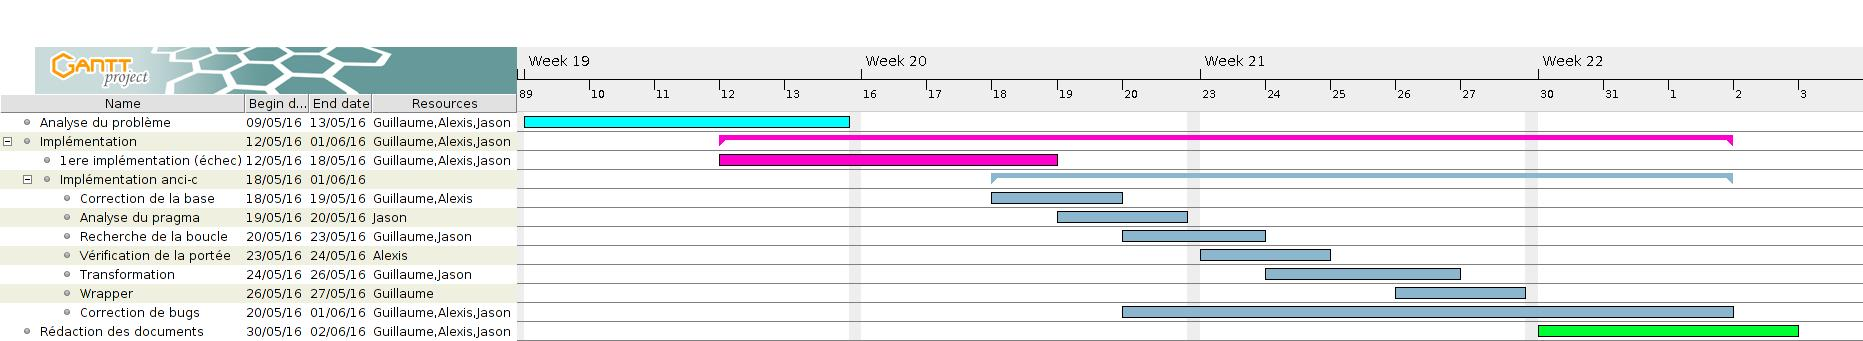
\includegraphics[scale=0.345]{Gantt/ganttPrev.jpg}
		\caption[Diagramme gantt de répartition des tâches]{Diagramme gantt de répartition des tâches}

  		\label{fig:gantt}
\end{figure}
	
\newpage
	
	
	
\printglossaries


\listoffigures

\lstlistoflistings



\section*{Bibliographie}
\begin{itemize}

\item https://github.com/dnoliver/tc-parser/tree/e3c06751c2bca8a9aaea8afe601a7ad05b3384a4
\item http://www.quut.com/c/ANSI-C-grammar-y.html
\item https://gcc.gnu.org/onlinedocs/gccint/Plugins-attr.html\#Plugins-attr

\end{itemize}
	

\newpage
	\section{Annexe}

	\subsection{Exemple}

	\begin{lstlisting}[
	caption=Code à CUDAiser (Exemple annexe),
    language=cpp,
]
int x1 = 2;
int y2 = 2;



#pragma cuda thread_loop(j) block_size(x1,y2) nbr_threads(16)
void sum(float *x, float *y, float *z, int size) {
 int i;
 for(i=0; i<size; ++i) {
   z[i] = x[i] + y[i];
 }
 int j;
 for(j=0; j<size; j++) {
    z[j] = x[j] + y[i];
 }
}


int main(int argc, char *argv[]) {
  int vector_size = 10;
  float h_x[vector_size], h_y[vector_size], h_z[vector_size];
  int i = 0;

  for (i = 0;i < vector_size; i++) {
		h_x[i] = i;
		h_y[i] = i;
	}

  sum(h_x, h_y, h_z, vector_size);

  return 0;
}
\end{lstlisting}

	\begin{lstlisting}[
	caption=Résultat de la CUDAisation (Exemple annexe),
    language=cpp,
]
int x1 = 2;
int y2 = 2;

__global__
void kernel_sum(float *x, float *y, float *z, int size)
{
	int i;
	for ( i = 0; i < size; ++i )
	{
		z[i] = x[i] + y[i];
	}
	int j = ((blockIdx.x * blockDim.x + threadIdx.x) * blockDim.y + threadIdx.y);
	if (j < size)
	{
		z[j] = x[j] + y[i];
	}
}
void sum(float *x, float *y, float *z, int size)
{
	 int nbr_thread_x = x1;
	 int nbr_thread_y = y2;
	 int nbr_block_x = (16 + x1*y2 - 1 ) / x1*y2;

	 kernel_sum <<< dim3(nbr_block_x) , dim3(nbr_thread_x, nbr_thread_y) >>> (x, y, z, size);
}
int main(int argc, char *argv[])
{
	int vector_size = 10;
	float h_x[vector_size], h_y[vector_size], h_z[vector_size];
	int i = 0;
	for ( i = 0; i < vector_size; i++ )
	{
		h_x[i] = i;
		h_y[i] = i;
	}
	sum(h_x, h_y, h_z, vector_size);
	return 0;
}

\end{lstlisting}

\subsection{Usage}

Usage: cudaparse [OPTION] [FILE]

Exemple: cudaparse main.c
\begin{itemize}

\item -x  		 Print an XML representation of the tree (build from ANSI-C).
\item -c  		 Print the C code with cuda kernel(s).
\item -o OUTPUT\_FILE 	 Save the result on a file, depend to the prints options (if none, store the c result).
\item -h 		 Print help informations.

\end{itemize}



\end{document}

